\documentclass[11pt, a4paper]{article}
\usepackage[utf8]{inputenc}
\usepackage[margin=.7in]{geometry}
\usepackage{listings}
\usepackage{setspace}
\usepackage{xcolor}
\usepackage{titlesec}
\usepackage{enumitem}
\usepackage{amssymb}
\usepackage{amsmath}
\usepackage{bm}
\usepackage{multicol}
\usepackage{graphicx}
\graphicspath{{./Figures/}}
\usepackage{color}
\usepackage{hyperref}
\hypersetup{
	colorlinks=true,
	linkcolor=blue,
	urlcolor=blue,
}
\titleformat*{\section}{\LARGE\bfseries\filcenter}
\titleformat*{\subsection}{\Large\bfseries}
\titleformat*{\subsubsection}{\large\bfseries}
\definecolor{codegreen}{rgb}{0,0.5,0}
\definecolor{codegray}{rgb}{0.5,0.5,0.5}
\definecolor{codered}{rgb}{0.78,0,0}
\definecolor{codepurple}{rgb}{0.58,0,0.68}
\definecolor{backcolour}{rgb}{0.95,0.95,0.92}
\lstdefinestyle{Pythonstyle}{
	language = Python,
    backgroundcolor=\color{backcolour},   
    commentstyle=\color{gray},
    keywordstyle=\color{codegreen},
    numberstyle=\tiny\color{codegray},
    stringstyle=\color{codered},
    basicstyle=\ttfamily\footnotesize,
    breakatwhitespace=false,         
    breaklines=true,                 
    captionpos=b,                    
    keepspaces=true,                 
    numbers=left,                    
    numbersep=5pt,                  
    showspaces=false,                
    showstringspaces=false,
    showtabs=false,                  
    tabsize=2,
    morekeywords = {as},
    keywordstyle = \color{codegreen}
}
\lstset{style=Pythonstyle}

\begin{document}
	\begin{titlepage}
		\begin{center} \Huge \textbf{Udacity: Intro to ML with PyTorch} \end{center}
		\tableofcontents
		\newpage
	\end{titlepage}
%%%% PAGE 1 %%%%

	\begin{spacing}{1.1}
	\section{Supervised Learning}
	\subsection{Linear Regression \href{https://scikit-learn.org/stable/modules/linear_model.html}{(doc)}}
	\textbf{Absolute Trick}: A point at $(p,q)$ with a line $y = w_1x + w_2$, we want to change the line to slowly move it towards the point. We want to do this by a small value $\alpha$ (learning rate), so our line become $\hat{y} = (w_1 + p\alpha)x + (w_2 + \alpha)$. \vspace*{2mm}\\
	\textbf{Square Trick}: Similar to the absolute trick, but we consider the offset of the point from the y-axis ($p$) and from the line ($q-q'$) where $q'$ is the \textit{estimated} $y$ point and $q$ is the actual $y$ point. So our line becomes $\hat{y} = (w_1 + p(q-q')\alpha)x + (w_2 + (q-q')\alpha)$\vspace*{2mm}\\
	\textbf{Mean Absolute Error}: the average of the sum of the distance between the estimate line value $\hat{y}$ and actual $y$ value, giving us the equation: $Error = \frac{1}{m} \sum_{i=1}^{m}|y-\hat{y}|$ \vspace*{2mm}\\
	\textbf{Mean Squared Error}: Similar to MAE, but we square the value instead which gives us a square near the value $y-\hat{y}$. This gives us the equation: $Error = \frac{1}{2m} \sum_{i=1}^{m}(y-\hat{y})^2$ \vspace*{2mm}\\
	\textbf{Gradient Step}: $w_i \rightarrow w_i - \alpha\frac{\partial}{\partial w_i}Error$ with $\frac{\partial}{\partial w_1}Error = -(y-\hat{y})x$ and $\frac{\partial}{\partial w_2}Error = -(y-\hat{y})$
	\begin{lstlisting}
	X : array of predictor features
	y : array of outcome values
	W : predictor feature coefficients
	b : regression function intercept
	learn_rate : learning rate
	
	yhat = np.matmul(X,W) + b # predicted values
	error = y-yhat
	W_new = W + learn_rate*np.matmul(error,X) # updated slope
	b_new = b + learn_rate*error.sum() # updated y-intercept \end{lstlisting}\vspace*{3mm}
	\textbf{Higher Dimensions}: $\hat{y} = w_1x_1 + w_2x_2 + ... + w_{n-1}x_{n-1} + w_n$ \vspace*{2mm}\\
	\textbf{Polynomial Regression}: Allows us to add degrees to our $x$ to better find our line.
	\begin{lstlisting}
	import numpy as np
	import pandas as pd
	from sklearn.preprocessing import PolynomialFeatures
	from sklearn.linear_model import LinearRegression
	
	train_data = pd.read_csv('data.csv')
	X = np.asarray(train_data['Var_X']).reshape((20,1))
	y = np.asarray(train_data['Var_Y']).reshape((20,1))
	
	poly_feat = PolynomialFeatures(degree=4) # 4th degree polynomial
	X_poly = poly_feat.fit_transform(X)
	
	poly_model = LinearRegression(fit_intercept=False).fit(X_poly, y) \end{lstlisting}\vspace*{3mm}
	\textbf{L1 Regularization}: adds the absolute value of the coefficients ($w_i$) to the error. This is computationally inefficient, better when data is sparse, gives us feature selection (makes irrelevant columns to 0). \vspace*{2mm}\\
	\textbf{L2 Regularization}: we add the square of the coefficients ($w_i$) to the error. This is computationally efficient, better for non-sparse data, doesn't have feature selection (treats all columns equally).  \vspace*{2mm}\\
	\textbf{$\mathbb{\lambda}$ Parameter}: determines how much impact the coefficients have on our total error. Choosing a large $\lambda$ leads to simpler models more while a small $\lambda$ leads to more complex models. \newpage
%%%% PAGE 2 %%%%

	\noindent We can train a Linear Regression model with L1 regularization applied to it by using the \href{https://scikit-learn.org/stable/modules/generated/sklearn.linear_model.Lasso.html}{Lasso model}.
	\begin{lstlisting}
	import pandas as pd
	from sklearn.linear_model import Lasso
	
	train_data = pd.read_csv('data.csv', header=None)
	X = train_data.iloc[:,:-1] # all rows, all colums up to last
	y = train_data.iloc[:,-1] # all rows, last column
	
	lasso_reg = Lasso().fit(X, y)
	
	reg_coef = lasso_reg.coef_
	print(reg_coef)
	# [ 0.  2.35793224  2.00441646 -0.05511954 -3.92808318  0.]	\end{lstlisting}\vspace*{3mm}
	\textbf{Feature Scaling}: a way of transforming your data into a common range of values (2 ways below).\vspace*{2mm}\\
	\textbf{Standardizing}: turning the column into a standard normal variable by computing $\frac{x-\mu}{\sigma}$ and is interpreted as the number of standard deviations each value is away from the mean (most common type).\vspace*{2mm}\\
	\textbf{Normalizing}: data is scaled between 0 and 1 by calculating $\frac{x-x.min}{x.max - x.min}$\vspace*{2mm}\\
	\textbf{Distance Based Metrics}: If an algorithm uses distance based metrics to predict, choosing some sort of feature scaling is necessary (such as for SVMs of k-nn).\vspace*{2mm}\\
	\textbf{When using Regularization}: we need all columns to have equal ranges so they are treated similar when calculating the penalty. We need features with small ranges and large ranges to have similar coefficients.
	\begin{lstlisting}
	import pandas as pd
	from sklearn.preprocessing import StandardScaler
	from sklearn.linear_model import Lasso
	
	train_data = pd.read_csv('data.csv', header=None)
	X = train_data.iloc[:, :-1]
	y = train_data.iloc[:, -1]
	
	scaler = StandardScaler()
	X_scaled = scaler.fit_transform(X)
	
	
	lasso_reg = Lasso().fit(X_scaled, y)
	
	reg_coef = lasso_reg.coef_
	print(reg_coef)
	# [0.   3.90753617   9.02575748  -0.   -11.78303187   0.45340137]	\end{lstlisting}\vspace*{3mm}
	Notice how after we scaled the features, the L1 regularization set the 1st and 4th columns coefficients to zero. Where when we did not standardize in the previous code, the L1 regularization set the 1st and 6th columns coefficients to zero. \newpage
%%%% PAGE 3 %%%%

	\subsection{Perceptron Algorithm}
	\textbf{Linear Boundaries}: we use a boundary line to determine how to classify the data, denoted by the equation $w_1x_1 + w_2x_2 + b = 0$ which we rewrite as $Wx+b = 0$ where $W=(w_1,w_2)$ and $x=(x_1,x_2)$. Note that we just take the dot product of $W\cdot x \implies w_1x_1 + w_2x_2$. We then classify the output of the boundary line by:
	$$\hat{y} = \begin{cases}
	1 \text{ if } Wx+b \geq 0\\
	0 \text{ if } Wx+b < 0
	\end{cases} $$
	\textbf{Higher Dimensions}: if we are working with $n$ columns, our boundary line becomes a $n-1$ dimensional hyperplane with the equation $w_1x_1 + w_2x_2 + ... + w_nx_n + b = 0 \implies Wx+b = 0$. The prediction works the same way as the linear boundary. Note that weights (W) is a (1xn) row vector, input (x) is a (nx1) column vector, and bias (b) is a (1x1) vector.\vspace*{2mm}\\
	\textbf{Basic Perceptrons}: We have our input nodes ($x_1,...,x_n$ and can also include our bias $b$) which are then multiplied by the corresponding weights ($w_1,...,w_n$), which are then inputted into a linear function node ($Wx+b$), and finally that input is sent to a step function node (determines if $\hat{y}$ is 1 or 0).\vspace*{2mm}\\
	\textbf{Updating the line}: In a 2D example, with point $(p,q)$, we can update the boundary line with the equation $ (w_1\pm\alpha p)x_1 + (w_2\pm\alpha q)x_2 + (b\pm\alpha*1)$. Note that $\pm$ depends on which way we move the line.
	\begin{lstlisting}
	def perceptronStep(X, y, W, b, learn_rate = 0.01):
		for i in range(len(X)): # go through all points
			yhat = prediction(X[i], W, b) # get predicted values
			if y[i] - yhat == 1: # if y=1 but yhat=0 (move line down)
				W[0] += learn_rate*X[i][0]
				W[1] += learn_rate*X[i][1]
				b +=learn_rate
			if y[i] - yhat == -1: # if y=0 but yhat=1 (move line up)
				W[0] -= learn_rate*X[i][0]
				W[1] -= learn_rate*X[i][1]
				b -=learn_rate    
		return W, b	\end{lstlisting} \vspace*{2mm}
	
	\subsection{Decision Trees \href{https://scikit-learn.org/stable/modules/tree.html}{(doc)}}
	\textbf{(Multiclass) Entropy}: $-\sum_{i=1}^np_i log_2(p_i)$ where $p_i$ is the probability for each class. Note that points with the same color will have zero entropy, so this is the ideal outcome for classification. \vspace*{2mm}\\
	\textbf{Information Gain}: Tells us how well our data is being classified (in a range between 0 and 1). The lower the information gain, the worse our model is doing as separating the data. The higher the information gain, the better our model is performing at classification. We have the formula: \\$IG = Entropy(Parent) - \Big[\frac{m}{m+n}Entropy(Child_1)+\frac{n}{m+n}Entropy(Child_2)\Big]$ \vspace*{2mm}\\
	\textbf{Important Hyperparameters for Decision Trees}: \vspace*{1mm} \\
	\textbf{Maximum depth}: the largest possible length between the root to a leaf, a tree of maximum length $k$ can have at most $2^k$ leaves. \vspace*{2mm}\\
	\textbf{Minimum samples to split}: numeric value ($m$) that says if a node doesn't have at least $m$ samples it can't split.\vspace*{2mm}\\
	\textbf{Minimum samples per leaf}: decides how many samples must be in each node. If it is an integer, then it is a sample size. If it is a float, it is a percentage of samples needed in a leaf. \vspace*{2mm}\\
	\textbf{WARNING}: Large depth often causes overfitting. Small depth can result in a very simple model, which may cause underfitting. Small minimum samples per split may result in overfitting. Large minimum samples may result in the tree not having enough flexibility to get built, and may result in underfitting. \newpage
%%%% PAGE 4 %%%%

	\begin{lstlisting}
	import pandas as pd
	import numpy as np
	from sklearn.model_selection import train_test_split
	from sklearn.tree import DecisionTreeClassifier
	from sklearn.metrics import accuracy_score
	import random
	random.seed(42)
	
	in_file = 'titanic_data.csv'
	full_data = pd.read_csv(in_file)
	
	outcomes = full_data['Survived'] # Labels
	features_raw = full_data.drop('Survived', axis = 1) # Remove label from features df
	
	features_no_names = features_raw.drop(['Name'], axis=1) # Remove names
	
	features = pd.get_dummies(features_no_names) # One-hot encoding
	features = features.fillna(0.0)
	
	len(features.columns) # 839
	# Note that we now have 839 columns instead of 11 since each ticket is a column
	# from the one-hot encoding (each ticket_number is now a column with all 0's 
	# expect for the person/row with the ticket, which will be a 1).
	
	X_train, X_test, y_train, y_test = train_test_split(features, outcomes, 
	                                                    test_size=0.2, random_state=42)
	
	model = DecisionTreeClassifier().fit(X_train, y_train)
	
	# Making predictions
	y_train_pred = model.predict(X_train)
	y_test_pred = model.predict(X_test)
	train_accuracy = accuracy_score(y_train, y_train_pred) # 1.0
	test_accuracy = accuracy_score(y_test, y_test_pred) # 0.8156
	# High training and lower test accuracy means we might be overfitting.
	
	# Tune the hyperparameters for new model to improve test score
	model_tune = DecisionTreeClassifier(max_depth=20, min_samples_leaf=6)
	model_tune.fit(X_train, y_train)
	tune_y_train_pred = model_tune.predict(X_train)
	tune_y_test_pred = model_tune.predict(X_test)
	tune_train_accuracy = accuracy_score(y_train, tune_y_train_pred)
	tune_test_accuracy = accuracy_score(y_test, tune_y_test_pred) 
	
	print('Train Acc: {}, Test Acc: {}'.format(tune_train_accuracy, tune_test_accuracy))
	# Train Acc: 0.8820224719101124, Test Acc: 0.8603351955307262 \end{lstlisting} \newpage
%%%% PAGE 5 %%%%

	\subsection{Naive Bayes \href{https://scikit-learn.org/stable/modules/naive_bayes.html}{(doc)}}
	\textbf{Naive Bayes}: a supervised machine learning algorithm that can be trained to classify data into multi-class categories. The probabilistic model computes the conditional probabilities of the input features and assigns the probability distributions to each of possible classes. \vspace*{2mm}\\
	\textbf{Bayes Theorem}: We have prior probabilities for a given problem, and after we know that event $B$ occurred, we can find the posterior probability with the formula $ P(A_j|B) = \frac{P(B|A_j)P(A_j)}{\sum P(B|A_i)P(A_i)}$\vspace*{2mm}\\
	\textbf{Naive Assumption}: $P(A\cap B) = P(A)P(B)$ meaning that the two events are independent. We assume this to be true even if it is not the case. \vspace*{2mm}\\
	\textbf{Conditional Probability (Proportional)}: $P(A|B_1,B_2,...,B_n) \propto P(B_1,B_2,...,B_n|A)P(A)$\vspace*{2mm}\\
	\textbf{Algorithm}: For an event A, we have $ P(A|B_1,B_2,...,B_n) \propto \frac{P(B_1|A)P(B_2|A)...P(B_n|A)P(A)}{P(B_1,B_2,...,B_n)}$  \vspace*{2mm}\\
	\textbf{Bag of Words (BoW)}: a collection of text data where we count the frequency of the words. \vspace*{2mm}\\
	\textbf{Accuracy}: the ratio of the number of correct predictions to the total number of predictions.\vspace*{2mm}\\
	\textbf{Precision}: a ratio of true positives to all positives (true+false positive).\vspace*{2mm}\\
	\textbf{Recall (Sensitivity)}: a ratio of true positives to all the words (true positives + false negatives).\vspace*{2mm}\\
	\textbf{F1 Score}:  is the weighted average of the precision and recall scores (between 0 and 1, higher better).
	\begin{lstlisting}
	import pandas as pd
	from sklearn.model_selection import train_test_split
	from sklearn.feature_extraction.text import CountVectorizer
	from sklearn.naive_bayes import MultinomialNB
	from sklearn.metrics import accuracy_score, precision_score, recall_score, f1_score
	
	# Read in data from table, add column names, specify seperator
	df = pd.read_table('smsspamcollection/SMSSpamCollection', sep='\t', 
	                   names=['label', 'sms_message'])
	
	# Convert labels to numerical encodings
	df['label'] = df.label.map({'ham':0, 'spam':1})
	
	X_train, X_test, y_train, y_test = train_test_split(df['sms_message'], df['label'], 
                                                      random_state=1)
	
	count_vector = CountVectorizer()
	# Note that CountVectorizer automatically converts to lowercase and ignores
	# all punctuation. We can add stop_words=English if we want to ignore
	# common english words (a, an, and) in our matrix.
	
	# Fit the training data and return the frequency matrix
	training_data = count_vector.fit_transform(X_train)
	
	# Transform testing data and return the matrix (don't fit testing data)
	testing_data = count_vector.transform(X_test)
	
	naive_bayes = MultinomialNB()
	naive_bayes.fit(training_data, y_train)
	predictions = naive_bayes.predict(testing_data)
	
	print('Accuracy score: ', format(accuracy_score(y_test, predictions))) # 0.98851
	print('Precision score: ', format(precision_score(y_test, predictions))) # 0.972067
	print('Recall score: ', format(recall_score(y_test, predictions))) # 0.94054
	print('F1 score: ', format(f1_score(y_test, predictions))) # 0.95604 \end{lstlisting} \newpage
%%%% PAGE 6 %%%%

	\subsection{Support Vector Machines (SVMs) \href{https://scikit-learn.org/stable/modules/generated/sklearn.svm.SVC.html}{(doc)}}
	\textbf{Classification Error}: we have a line separating our data points into groups, $Wx+b = 0$, and we want to add two more lines called the \textit{margin}. The line above has equation $Wx+b = 1$ and the line below has equation $Wx+b = -1$. We then assign points error based on where they are in respect to the margin:
	\begin{center}
	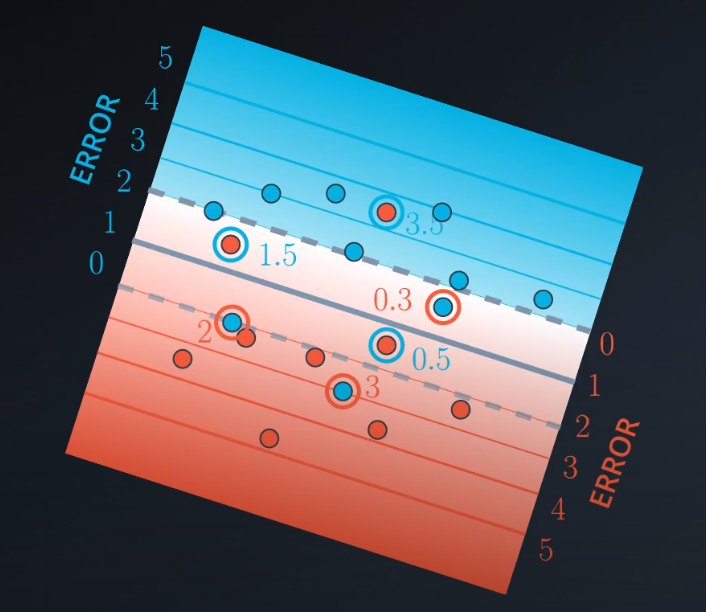
\includegraphics[scale=.3]{SVM}
	\end{center}
	\textbf{Classification Error}: we take the absolute value of all misclassified points and add them together. \vspace*{2mm}\\
	\textbf{Margin}: we want a small error if the margin is large, and a large error if the margin is small. We can determine the size of the margin by $\frac{2}{|W|}$ (2 divided by the norm of $W$). \vspace*{2mm}\\
	\textbf{Margin Error}: $|W|^2$ (note this is the same value given by L2 regularization). \vspace*{2mm}\\
	\textbf{Error Function}: we want Error = Classification Error + Margin Error, which we will minimize using gradient descent. \vspace*{2mm}\\
	\textbf{The C Parameter}: Error = C*Classification Error + Margin Error. It is a constant we use to determine the influence of the classification error. Large C means focus on classifying points (smaller margin), small C means focus on margin error (makes more classification errors).\vspace*{2mm}\\
	\textbf{Linear Kernel}: we separate our data using a linear line (doesn't work well when data is complicated).\vspace*{2mm}\\
	\textbf{Polynomial Kernel}: we separate our data using circles, hyperbolas, parabolas, and many more boundaries by adding more dimensions to our data to classify it. The degree of the polynomial determines what kind of boundaries we can create.\vspace*{.5mm}\\
	ex: (degree 2) $\mathbb{E}^2 \rightarrow \mathbb{E}^5: (x,y) \rightarrow(x,y,x^2,xy,y^2)$. We map our points (x,y) to a higher dimensions which allows us to create degree 2 functions. We then find a boundary hyperplane and map this back to a 2nd degree polynomial boundary (think of a paraboloid in 3D mapping back to a circle in 2D). \vspace*{2mm}\\
	\textbf{RBF Kernel}: We build mountain ranges (radial basis functions) on top of our point to find boundaries to group the data. The plane that intersects the paraboloids is the projection that determine the boundaries. The $\gamma$ hyperparameter can be tuned to determine the width of the curve, with a small $\gamma$ giving us a wide curve and a large $\gamma$ giving us a narrow curve.
	\begin{lstlisting}
	from sklearn.svm import SVC
	from sklearn.metrics import accuracy_score
	
	data = np.asarray(pd.read_csv('data.csv', header=None)) 
	X = data[:,0:2] # features
	y = data[:,2] # labels
	
	model = SVC(kernel='rbf', gamma=27).fit(X,y)
	
	y_pred = model.predict(X)
	acc = accuracy_score(y, y_pred)
	\end{lstlisting} \newpage
%%%% PAGE 7 %%%%

	\subsection{Ensemble Methods \href{https://scikit-learn.org/stable/modules/ensemble.html}{(doc)}}
	\textbf{Bias}: when a model has high bias, this means that it doesn't do a good job of bending to the data. One example is linear regression, which fits a straight line no matter how the data is shaped (but has a low variance).\vspace*{2mm}\\
	\textbf{Variance}: when a model has high variance, this means that it changes drastically to meet the needs of every point in our dataset. One example are decision trees, which will attempt to split every point into its own branch if possible (but has low bias).\vspace*{2mm}\\
	\textbf{High Bias, Low Variance}: models tend to underfit data, as they are not flexible (linear models).\vspace*{2mm}\\
	\textbf{High Variance, Low Bias}: models tend to overfit data, as they are too flexible (decision trees). \vspace*{2mm}\\
	\textbf{Randomness}: introduction of randomness to high variance algorithms to combats the tendency of these algorithms to overfit the data. \vspace*{2mm}\\
	\textbf{Bootstrap}:  sampling the data with replacement and fitting your algorithm to the sampled data. \vspace*{2mm}\\
	\textbf{Boosting}: Random sampling with replacement over weighted data. \vspace*{2mm}\\
	\textbf{Random Forests}: take a subset of the columns and build a decision tree from them, then repeat this process multiple times. We then use each tree to predict, and pick the most occurring outcome.\vspace*{2mm}\\
	\textbf{Bagging}: take subsets of the data, create one-node decision trees to find a boundary for each subset, then take the overlap of the boundaries to determine the final boundary line (bootstrapping). \vspace*{2mm}\\
	\textbf{AdaBoost}: we assign weights to each points, and we want to minimize the sum of the weights on the incorrectly classified points. We then increase the weights (by $\frac{\sum correct\, weights}{\sum incorrect\, weights}$) of the misclassified points and create a new boundary line. We continue this process for multiple models. \vspace*{.7mm}\\
	Once we have our models, we assign weight to the models to determine the influence they have in our final boundary, which can be calculated by $weight = ln(\frac{\#\, correct}{\#\, incorrect})$
	\begin{lstlisting}
	# NOTE: we are using the testing and training data from the Naive Bayes
	# section, so refer to that to see data preprocessing steps
	
	from sklearn.ensemble import AdaBoostClassifier
	from sklearn.ensemble import BaggingClassifier
	from sklearn.ensemble import RandomForestClassifier
	from sklearn.metrics import accuracy_score, precision_score, recall_score, f1_score
	
	bag_model = BaggingClassifier(n_estimators=200).fit(training_data, y_train)
	rf_model = RandomForestClassifier(n_estimators=200).fit(training_data, y_train)
	ada_model = AdaBoostClassifier(n_estimators=300, learning_rate=0.2)
	ada_model.fit(training_data, y_train)
	
	bag_ypred = bag_model.predict(testing_data)
	rf_ypred = rf_model.predict(testing_data)
	ada_ypred = ada_model.predict(testing_data)
	
	# General Format for printing evaluation metrics (scoring model)
	print('Accuracy score: ', format(accuracy_score(y_true, preds)))
	print('Precision score: ', format(precision_score(y_true, preds)))
	print('Recall score: ', format(recall_score(y_true, preds)))
	print('F1 score: ', format(f1_score(y_true, preds)))	
	\end{lstlisting} \vspace*{3mm}
	NOTE: the \textit{base\_estimator} parameter for AdaBoost and Bagging allows you to choose the weak leaner model to be used in the classification process.	\newpage
%%%% PAGE 8 %%%%

	\subsection{Model Evaluation Metrics}
	\subsubsection{Classification Metrics (\href{https://en.wikipedia.org/wiki/Precision\_and\_recall\#Definition\_(classification\_context)}{formulas})}
	\textbf{Confusion Matrix}: a table that tells us the True Positive, False Negatives, False Positive, and True Negatives (left to right, top to bottom).\vspace*{2mm}\\
	\textbf{Error Types}: False Positives are classified as \textit{Type 1 Error}, False Negative are \textit{Type 2 Error}.\vspace*{2mm}\\
	\textbf{Accuracy}: used to compare models, it tells us the proportion of observations we correctly labeled (don't use if classes are imbalanced).\vspace*{2mm}\\
	\textbf{Precision}: focuses on \textit{predicted} positive values, helps determine if you are doing a good job of predicting the positive values, as compared to predicting negative values as positive. Avoiding false positives.  \vspace*{2mm}\\
	\textbf{Recall}: focuses on the \textit{actual} positive values, determines if you are doing a good job of predicting the positive values without regard of how you are doing on the actual negative values. Avoiding false negatives. \vspace*{2mm}\\
	\textbf{F1 Score}: the harmonic mean (less than regular mean), found by $2*\frac{Precision*Recall}{Precision+Recall}$ (care equally about both the positive and negative cases). \vspace*{2mm}\\
	\textbf{$F_\beta$ Score}: If we want our model to focus more on precision than recall (such as spam filtering), we can use a smaller $\beta$. If we want our model to focus more on recall than precision (such as medical diagnosis), we can use a larger $\beta$. The formula is $F_\beta = (1+\beta^2) \frac{precision*recall}{\beta^2 * precision + recall}$\vspace*{2mm}\\
	\textbf{ROC Curve \& AUC}: By finding different thresholds for our classification metrics, we can measure the area under the ROC curve. When the AUC is closer to 1, the better your model is performing.
	\begin{lstlisting}
	# Again, we are using the data from the Naive Bayes section, so refer
	# back to that to see the data preprocessing steps
	
	from sklearn.naive_bayes import MultinomialNB
	from sklearn.metrics import accuracy_score, precision_score, recall_score, f1_score, 
	                            fbeta_score
	from sklearn.ensemble import BaggingClassifier, RandomForestClassifier, 
	from sklearn.svm import SVC
	
	naive_bayes = MultinomialNB().fit(training_data, y_train)
	bag_mod = BaggingClassifier(n_estimators=200).fit(training_data, y_train)
	rf_mod = RandomForestClassifier(n_estimators=200).fit(training_data, y_train)
	svm_mod = SVC().fit(training_data, y_train)
	
	nb_preds = naive_bayes.predict(testing_data)
	bag_preds = bag_mod.predict(testing_data)
	rf_preds = rf_mod.predict(testing_data)
	svm_preds = svm_mod.predict(testing_data)
	
	def metric_scores(actual, preds, model, model_name):
		print('Accuracy for ' + model_name + ' : {}'.format(accuracy_score(actual, preds)))
		print('Precision ' + model_name + ' : {}'.format(precision_score(actual, preds)))
		print('Recall for ' + model_name + ' : {}'.format(recall_score(actual, preds)))
		print('F1 for ' + model_name + ' : {}'.format(f1_score(actual, preds)))
		print('\n')
		return None
	
	metric_scores(y_test, nb_preds, naive_bayes, 'Naive Bayes')
	metric_scores(y_test, bag_preds, bag_mod, 'Bagging')
	metric_scores(y_test, rf_preds, rf_mod, 'Random Forest')
	metric_scores(y_test, svm_preds, svm_mod, 'SVM')
	# Running this, Naive Bayes performed best for all expect precision (rf_model)
	fbeta_score(y_test, nb_preds, beta=1) # same output as F1 score since beta=1 \end{lstlisting} \newpage
%%%% PAGE 9 %%%%

	\begin{lstlisting}
	from itertools import cycle
	from sklearn.metrics import roc_curve, auc, roc_auc_score
	from scipy import interp
	
	def build_roc_auc(model, X_train, X_test, y_train, y_test):
		y_preds = model.fit(X_train, y_train).predict_proba(X_test)
		# Compute ROC curve and ROC area for each class
		fpr = dict()
		tpr = dict()
		roc_auc = dict()
		for i in range(len(y_test)):
			fpr[i], tpr[i], _ = roc_curve(y_test, y_preds[:, 1])
			roc_auc[i] = auc(fpr[i], tpr[i])
		
		# Compute micro-average ROC curve and ROC area
		fpr["micro"], tpr["micro"], _ = roc_curve(y_test.ravel(), y_preds[:, 1].ravel())
		roc_auc["micro"] = auc(fpr["micro"], tpr["micro"])
		
		plt.plot(fpr[2], tpr[2], color='darkorange', lw=2, 
		         label='ROC curve (area = %0.2f)' % roc_auc[2])
		plt.plot([0, 1], [0, 1], color='navy', lw=2, linestyle='--')
		plt.xlim([0.0, 1.0])
		plt.ylim([0.0, 1.05])
		plt.xlabel('False Positive Rate')
		plt.ylabel('True Positive Rate')
		plt.title('Receiver operating characteristic example')
		plt.show();
		
		return roc_auc_score(y_test, np.round(y_preds[:, 1])) \end{lstlisting} \vspace*{1mm}
	\subsubsection{Regression Metrics}
	\textbf{Mean Absolute Error (MAE)}: a useful metric to optimize on when the value you are trying to predict follows a skewed distribution (not as much influence from outliers as MSE). The optimal value for this technique is the median value. \vspace*{2mm}\\
	\textbf{Mean Squared Error (MSE)}: most used metric for optimization (impacted by outliers and skew), it is differentiable and can be used better for gradient descent. The optimal value is the mean. \vspace*{2mm}\\ 
	\textbf{R2 Score}: interpreted as the `amount of variability' captured by a model. Minimizing MSE will maximize R2, which is good since we want this score to be as close to 1 as possible.
	\begin{lstlisting}
	# Import all regression models
	from sklearn.linear_model import LinearRegression
	from sklearn.ensemble import RandomForestRegressor, AdaBoostRegressor
	from sklearn.tree import DecisionTreeRegressor
	from sklearn.metrics import r2_score, mean_absolute_error, mean_squared_error
	
	def reg_metrics(actual, preds, model, model_name):
		print('R2 ' + model_name + ' : {}'.format(r2_score(actual, preds)))
		print('MAE ' + model_name + ' : {}'.format(mean_absolute_error(actual, preds)))
		print('MSE ' + model_name + ' : {}'.format(mean_squared_error(actual, preds)))
		print('\n')
		return None	\end{lstlisting} \vspace*{2mm}
	Using the Boston housing dataset, if were were to fit and predict on all of the models above, we would see that the RandomForestRegressor performs the best on all evaluation metrics. \newpage
%%%% PAGE 10 %%%%

	\subsection{Training and Tuning}
	\textbf{Underfitting}: making our model too simple, leading to bad accuracy on the training and testing set (an error due to high bias). Does not generalize well to new data. \vspace*{2mm}\\
	\textbf{Overfitting}: making our model too complicated, leading to higher training set accuracy but low testing set accuracy (an error due to high variance). Does not generalize well to new data. \vspace*{2mm}\\
	\textbf{K-Fold Cross Validation}: splitting our data $k$ time into training and testing sets to train and evaluate our model on different data combinations, so we don't lose some of the data. \vspace*{2mm}\\
	\textbf{Learning Curves}: In a model that is underfitting, the training and CV error converge at a high error. In a model that is overfitting, the training and CV error do not converge. In a good model, the training and CV error will converge at a low error point. \vspace*{2mm}\\
	\textbf{Grid Search}: combines all specified combinations of hyperparameters to find the best model. We then pick the one with the highest F1 score as our model and use a testing set to verify.
	\begin{lstlisting}
	import pandas as pd
	import numpy as np
	from sklearn.datasets import load_diabetes
	from sklearn.model_selection import train_test_split, RandomizedSearchCV
	from sklearn.metrics import accuracy_score, precision_score, recall_score, f1_score
	from sklearn.ensemble import RandomForestClassifier, AdaBoostClassifier
	import matplotlib.pyplot as plt
	from sklearn.svm import SVC
	import seaborn as sns
	sns.set(style="ticks")
	
	diabetes = pd.read_csv('diabetes.csv')
	
	# Data Analysis
	diabetes.describe() # see summary statistics for each column
	diabetes.isna().any() # (0) - find number of NA values (by column) 
	diabetes['Outcome'].sum()/len(diabetes) # (0.35) - proportion of diabetes outcomes
	diabetes['Age'].value_counts().hist() # right-skewed data
	diabetes['Glucose'].hist() # approx normal distribution
	sns.heatmap(diabetes.corr(), annot=True, cmap="YlGnBu"); # correlation heatmap
	
	y = diabetes['Outcome']
	X = diabetes.drop(columns='Outcome', axis=1)
	X_train, X_test, y_train, y_test = train_test_split(X, y, test_size=0.2, 
	                                                    random_state=42)
	
	# Build a RandomForestClassifier and use RandomizedSeach to find best params
	clf_rf = RandomForestClassifier()
	
	param_dist = {"max_depth": [3, None],
				"n_estimators": list(range(10, 200)),
				"max_features": list(range(1, X_test.shape[1]+1)),
				"min_samples_split": list(range(2, 11)),
				"min_samples_leaf": list(range(1, 11)),
				"bootstrap": [True, False],
				"criterion": ["gini", "entropy"]}
	
	random_search = RandomizedSearchCV(clf_rf, param_distributions=param_dist)
	random_search.fit(X_train, y_train)
	
	rf_preds = random_search.best_estimator_.predict(X_test)
	print('F1 Score: {}'.format(f1_score(y_test, rf_preds))) # 0.6847 \end{lstlisting} \newpage
%%%% PAGE 11 %%%%

	\begin{lstlisting}
	# Build a AdaBoostClassifier and use RandomizedSeach to find best params
	ada = AdaBoostClassifier()
	
	parameters = {'n_estimators': list(range(50, 275, 25)),
			'learning_rate': [0.001, 0.01, 0.1, 0.2, 0.3, 0.4, 0.5, 1, 2, 5, 10, 15]}

	ada_random = RandomizedSearchCV(ada, param_distributions=parameters)
	ada_random.fit(X_train, y_train)

	ada_preds = ada_random.best_estimator_.predict(X_test)
	print('F1 Score: {}'.format(f1_score(y_test, ada_preds))) # 0.6729
	
	# Plotting feature importance
	features =  diabetes.columns[:-1]
	importances = random_search.best_estimator_.feature_importances_
	indices = np.argsort(importances)
	
	plt.title('Feature Importance (Random Forest Classifier)')
	plt.barh(range(len(indices)), importances[indices], color='b', align='center')
	plt.yticks(range(len(indices)), [features[i] for i in indices])
	plt.xlabel('Relative Importance')
	plt.show() # Glucose, BMI, and Age were the top 3 features \end{lstlisting} \vspace*{3mm}
	Note that these features ranking were very similar to the heatmap that was made (except for pregnancies, which turned out to be the least influential feature). \vspace*{2mm}\\
	In this case study, we looked at predicting diabetes for 768 patients.  There was a reasonable amount of class imbalance with just under 35\% of patients having diabetes.  There were no missing data, and initial looks at the data showed it would be difficult to separate patients with diabetes from those that did not have diabetes. \vspace*{2mm}\\
	Two advanced modeling techniques were used to predict whether or not a patient has diabetes.  The most successful of these techniques proved to be the RandomForestClassifier, which had the following metrics: \\
	Accuracy score for random forest : 0.7727272727272727\\
	Precision score random forest : 0.6785714285714286\\
	Recall score random forest : 0.6909090909090909\\
	F1 score random forest : 0.6846846846846847\vspace*{1mm}\\
	Based on the initial look at the data, it is unsurprising that Glucose, BMI, and Age were important in understanding if a patient has diabetes. It was surprising seeing that pregnancy looked to be correlated in the initial heatmap, but turned out to be the least important feature in our final model. This could have been due to its high correlation with the Age feature. \newpage
%%%% PAGE 12 %%%%
	
	\section{Deep Learning}
	\subsection{Neural Networks}
	NOTE: refer back to Perceptron Algorithm section (1.2) for basic building blocks. \vspace*{2mm}\\
	\textbf{Error Function}: tells us the distance we are from the points, assigning more weight to the misclassified points and less to the correctly classified points. This should be continuous (not discrete). \vspace*{2mm}\\
	\textbf{Continuous Predictions}: we now want to classify points based on probability since we are working in the continuous world. Using the \textit{Sigmoid Function}, we classify all points with probability $<$ 0.5 as 0 and all points with probability $>$ 0.5 as 1. \vspace*{2mm}\\
	\textbf{Sigmoid Function (Binary)}: we now classify points as $\hat{y} = \sigma(Wx+b)$. The formula is $\frac{1}{1+e^{-x}}$ and will gives us a probability, which we classify based on a boundary line of 0.5. \vspace*{2mm}\\
	\textbf{Softmax Function (Multi-class)}: We apply the softmax function, $\frac{e^{Z_i}}{e^{Z_1}+...+e^{Z_n}}$, to all of the linear function scores ($Wx+b$) to find the probability for each class.
	\begin{lstlisting}
	def softmax(L):
		# Takes a list of numbers and returns the softmax values for each
		p_class = []
		for z in L:
			p_class.append(np.exp(z)/np.sum(np.exp(L)))
		return p_class
	\end{lstlisting} \vspace*{2mm}
	\textbf{One-Hot Encoding}: for labels, create a column for each label option and assign a 1 if it is the corresponding label, otherwise assign it a 0. In general, we will have $n$ columns for $n$ labels.\vspace*{2mm}\\
	\textbf{Cross-Entropy}: we want to maximize our probabilities that each point is correctly classified, which will minimize the error function. We sum across all of our probabilities, taking the -log() of each. If our point probability is near 1, it will have a small value. If our probability is near 0, it will have a larger value. This means a good model will give us a low cross-entropy. Points that are correctly classified have small errors, and points that are misclassified will have large errors.	
	\begin{lstlisting}
	def cross_entropy(Y, P):
		# Y are our labels, P is our probabilities
		Y = np.float_(Y)
		P = np.float_(P)
		return -np.sum(Y*np.log(P) + (1-Y)*np.log(1-P))
	\end{lstlisting} \vspace*{2mm}
	\textbf{Binary Cross-Entropy}: $E(W,b) = -\frac{1}{m} \sum_{i=1}^m y_i\,  ln(\hat{y}_i) + (1-y_i)ln(1-\hat{y}_i)$ where $\hat{y}_i = \sigma(Wx^{(i)}+b)$  \vspace*{2mm}\\
	\textbf{Multi-Class Cross-Entropy}: $E(W,b) = -\frac{1}{m} \sum_{i=1}^m \sum_{j=1}^n y_{ij}\, ln(\hat{y}_{ij})$ where $\hat{y}_{ij} = \sigma(Wx^{(ij)} + b)$  \vspace*{2mm}\\
	\textbf{Gradient Descent}: We want to minimize of size of $E(W,b)$ by taking steps downwards, which we can do by taking $\nabla E = [\frac{\partial E}{\partial w_1},..., \frac{\partial E}{\partial w_n}, \frac{\partial E}{\partial b}] = -(y-\hat{y})(x_1,...,x_n,1)$ and then taking a step in the direction $-\alpha\nabla E$ since we want to move down scaled by a learning rate $\alpha$. We then updated parameters as follows: $w_i' = w_i - \alpha \frac{\partial E}{\partial w_i} \implies w_i' = w_i + \alpha(y-\hat{y})x_i $ and $b' = b - \alpha \frac{\partial E}{\partial b} \implies b' = b + \alpha(y-\hat{y})$. We repeat this for a certain number of epochs until we minimize error. 
	\begin{lstlisting}
	# Activation (sigmoid) function
	def sigmoid(x):
		return 1/(1+np.exp(-x))
	
	# Output (prediction) formula
	def output_formula(features, weights, bias):
		return sigmoid(np.dot(features,weights) + bias)	\end{lstlisting} \newpage
	
%%%% PAGE 13 %%%%
	\begin{lstlisting}
	# Error (log-loss) formula
	def error_formula(y, output):
		return -y*np.log(output) - (1-y)*np.log(1-output)
	
	# Gradient descent step
	def update_weights(x, y, weights, bias, learnrate):
		output = y-output_formula(x,weights,bias)
		weights = weights + learnrate*output*x
		bias = bias + learnrate*output
		return weights, bias 
	\end{lstlisting} \vspace*{2mm}
	\textbf{General Neural Network}: We have our input layer ($x_1,...,x_n$), our hidden layer (set of linear models created from the input), and our output layer (a combination of linear models to create a non-linear model). If we have $n$ inputs, then our output will live in $n$ dimensions.\vspace*{2mm}\\
	\textbf{Deep Neural Networks}: We have an input layer, our linear models combine to create non-linear models in the hidden layers, and we combine these to output an advance non-linear model.\vspace*{2mm}\\
	\textbf{Multi-Class Networks}: If we have $n$ classes, then we have the same general architecture, but our output with have $n$ nodes that each output a probability for the class. We then take the highest probability as the class label.\vspace*{2mm}\\
	\textbf{Feedforward}: the process neural networks use to turn the input into an output. We take a vector of input features, and apply a sequence of linear models and sigmoid functions, which then output a probability of which label to assign to the prediction. Say we have a network with 1 input layer, 2 hidden layers, and an output layer. We take the output of the previous layer and use it as in input for our sigmoid of the current layer. We calculate $\hat{y}$ as: $\hat{y} = \sigma \circ W^{(3)} \circ \sigma \circ W^{(2)} \circ \sigma \circ W^{(1)}(x)$ \vspace*{2mm}\\
	\textbf{Error Function}: $E(W) = -\frac{1}{m} \sum_{i=1}^m y_i\,  ln(\hat{y}_i) + (1-y_i)ln(1-\hat{y}_i)$ where $\hat{y}_i$ is defined above. \vspace*{2mm}\\
	\textbf{Backpropagation}: similar to gradient descent, we use this to update weights and get better predictions. However, keras handles this for us for the most part. To know: error term = $(y-\hat{y})\sigma'(x)$ \vspace*{1mm}
	
	\subsection{Implementing Gradient Descent (NumPy)}
	\textbf{Mean Square Error}: the mean of the squares of the differences between the predictions and the labels.\vspace*{2mm}\\
	\textbf{Sum of Squared Errors (SSE)}: $E = \frac{1}{2} \sum_{\mu} \sum_j [y_j^{\mu} - \hat{y}_j^{\mu}]^2$ where variable $j$ represents the output units of the network. The other sum over $\mu$ is a sum over all the data points. Adding these two errors and dividing by 2 gives us SSE. \vspace*{2mm}\\	
	\textbf{Momentum}: used to avoid ending up in a local minima instead of a global minima when performing gradient descent.\vspace*{2mm}\\
	\textbf{Weight Matrix}: Each row in the matrix will correspond to the weights leading out of a single input unit ($i$), and each column will correspond to the weights leading in to a single hidden unit ($j$). So for a network with 3 inputs and 2 hidden layers, we will have a 3x2 matrix of weights, which we index at $w_{ij}$.\vspace*{2mm}\\
	\textbf{Input matrix}: we need to be sure our dimensions match. The columns in the input must match the rows in the hidden layer.\vspace*{2mm}\\
	\textbf{Hidden Layer Input}: we take the dot product of the input vector with the corresponding column of the weight matrix for the correct hidden layer unit. \newpage	
%%%% PAGE 14 %%%%

	\begin{lstlisting}
	def sigmoid(x):
		return 1/(1+np.exp(-x))
	
	# Network size
	N_input = 4
	N_hidden = 3
	N_output = 2
	
	np.random.seed(42)
	X = np.random.randn(4)
	
	weights_input_to_hidden = np.random.normal(0, scale=0.1, size=(N_input, N_hidden))
	weights_hidden_to_output = np.random.normal(0, scale=0.1, size=(N_hidden, N_output))
	
	hidden_layer_in = np.dot(X, weights_input_to_hidden) # 1x4*4x3 = 1x3
	hidden_layer_out = sigmoid(hidden_layer_in) # 1x3 matrix passed through sigmoid
	
	output_layer_in = np.dot(hidden_layer_out, weights_hidden_to_output) # 1x3*3x2 = 1x2
	output_layer_out = sigmoid(output_layer_in) # 1x2 matrix passed through sigmoid
	\end{lstlisting} \vspace*{2mm}
	
	\subsection{Training Neural Networks}
	\textbf{Underfitting}: an error due to high bias (too simple), low accuracy on both training and test sets.\vspace*{2mm}\\
	\textbf{Overfitting}: an error due to high variance (too specific), low test accuracy but high training accuracy. \vspace*{2mm}\\
	\textbf{Model Choice}: tend to the side of more complicated models, and apply techniques to prevent overfitting.\vspace*{2mm}\\
	\textbf{Model Complexity Graph}: plots number of epochs against error, shows us when we start to overfit data as our testing error goes from decreasing to increasing when our training error is still decreasing.\vspace*{2mm}\\
	\textbf{Early Stopping}: perform gradient descent until the testing error stops decreasing and starts increasing, at which point we stop training. \vspace*{2mm}\\
	\textbf{Regularization}: large coefficients leads to our model overfitting, so we want to penalize large weights. We can redefine our error function using L1 or L2 regularization. \vspace*{2mm}\\
	\textbf{L1 Regularization}: $E = -\frac{1}{m} \sum_{i=1}^m(1-y_i)ln(1-\hat{y}_i) + y_i\, ln(\hat{y}_i) + \lambda(|w_1| + ... + |w_n|)$\vspace*{2mm}\\
	\textbf{When to use L1}: using L1 we end up with sparse vectors (0,1,1,0,0,...) and small weights go to 0. If we want to reduce the number of weights and choose the best features for our model, this is a good option.\vspace*{2mm}\\
	\textbf{L2 Regularization}: $E = -\frac{1}{m} \sum_{i=1}^m(1-y_i)ln(1-\hat{y}_i) + y_i\, ln(\hat{y}_i) + \lambda(w_2^2 + ... + w_n^2)$\vspace*{2mm}\\
	\textbf{When to use L2}: using L2 keeps all weights even if they are small. Normally this gives better results when training a model (smaller error), so this is the most common.\vspace*{2mm}\\
	\textbf{Dropout}: some nodes have larger weights and more influence in our models training, so we choose a number of nodes to turn off randomly when training for each epoch (different each time). We assign a probability to each node of it being dropped when training.\vspace*{2mm}\\
	\textbf{Random Restart}: when performing gradient descent, we can get stuck in a local minima instead of a global one. To avoid this, we can start from a few different random place and perform gradient descent from all of them (higher probability of finding global minima). \vspace*{2mm}\\
	\textbf{ReLu Activation}: rectified linear unit, returns 0 if x is negative, otherwise returns x. The derivative is 1 is the number is positive, otherwise it is 0. \newpage
%%%% PAGE 15 %%%%

	\noindent \textbf{Batch Gradient Descent}: we run all of our data through the network for each epoch, calculate the gradient for all points, and move in the given direction.  \vspace*{2mm}\\
	\textbf{Stochastic Gradient Descent}: take small subsets (batches) of our data and run them through the network, calculate the gradient for the subset of points and move in the given direction. Repeat this process for each batch of our data until we have gone through them all (this is considered one epoch). \vspace*{2mm}\\
	\textbf{Learning Rate}: a large learning rate means big steps, which could go over our minima. A small learning rate means small steps, but longer training time. We can use a \textit{decreasing learning rate} to change over time as we get closer to a minima.\vspace*{2mm}\\
	\textbf{Momentum}: we want to take the average of the last few steps to determine the next step size. We multiply this by a constant, $\beta$, between 0 and 1 so more recent steps have more influence than farther back steps. $STEP(n) = STEP(n) + \beta STEP(n-1) + \beta^2 STEP(n-2)+...$\vspace*{3mm}
	
	\subsection{Deep Learning with PyTorch}
	\subsubsection{Building Neural Networks}
	\textbf{Tensors}: the fundamental data structure for neural networks, similar to vectors and matrices.\vspace*{2mm}\\
	\textbf{Reshaping Tensors}: we need input columns to match weights row. We can use .view(r,c) to do this.\vspace*{2mm}\\
	\textbf{NumPy to Torch}: we often prepare data with NumPy and then want to convert it into tensors. The memory is shared between the arrays, so changing one will result in the other changing as well.
	\begin{lstlisting}
	a = np.random.rand(4,3)
	b = torch.from_numpy(a)
	b.mul_(2)
	# Note that now 'a' has been multiplied by 2 as well
	\end{lstlisting} \vspace*{2mm}
	\textbf{MNIST Dataset}: a collection of greyscale handwritten digits from 0-9. We read them in with a batch size of 64, and the trainloader contains batches of 64 images that we will get during each iteration (they will also be shuffled). 
	\begin{lstlisting}
	import numpy as np
	import torch
	import matplotlib.pyplot as plt
	%matplotlib inline
	%config InlineBackend.figure_format = 'retina'
	from torchvision import datasets, transforms
	
	# Define a transform to normalize the data
	transform = transforms.Compose([transforms.ToTensor(), 
	                                transforms.Normalize((0.5,), (0.5,)),])
	
	# Download and load the training data
	trainset = datasets.MNIST('~/.pytorch/MNIST_data/', download=True, train=True, 
	                          transform=transform)
	trainloader = torch.utils.data.DataLoader(trainset, batch_size=64, shuffle=True)
	
	dataiter = iter(trainloader) # grab first batch, used only to inspect some images
	images, labels = dataiter.next()
	print(images.shape) # torch.Size([64, 1, 28, 28]) [batch, color, height, width]
	\end{lstlisting} \newpage
%%%% PAGE 16 %%%%

	\noindent \textbf{PyTorch Functional Module}: we can define a model in PyTorch by using the functional library. We will build a 3 layer NN that uses a ReLU activation function and outputs to a softmax. We also want to initialize our weights and biases (this is done automatically, but we can also do it manually with custom values).
	\begin{lstlisting}
	import torch.nn.functional as F
	
	class Network(nn.Module): # subclass of nn.Module
		def __init__(self):
			super().__init__() # defines architecture
			# Define input layers (Wx+b) for two hidden and one output layer
			self.hidden1 = nn.Linear(784, 128) # initial input
			self.hidden2 = nn.Linear(128, 64) # input from first hidden layer
			self.output = nn.Linear(64, 10) # Output layer, 10 units - one for each digit
		
		def forward(self, x):
			x = F.relu(self.hidden1(x)) # Hidden layer1 with relu activation
			x = F.relu(self.hidden2(x)) # Hidden layer2 with relu activation
			x = F.softmax(self.output(x), dim=1) # Output layer with softmax activation
			return x
	
	model = Network()
	model
	# Network(
	# (hidden1): Linear(in_features=784, out_features=128, bias=True)
	# (hidden2): Linear(in_features=128, out_features=64, bias=True)
	# (output): Linear(in_features=64, out_features=10, bias=True)
	# )
	
	# Set biases to all zeros (note that this is done inplace)
	model.hidden1.bias.data.fill_(0)
	# sample from random normal with standard dev = 0.01 (note that this is done inplace)
	model.hidden1.weight.data.normal_(std=0.01)	
	\end{lstlisting} \vspace*{1mm}
	\textbf{PyTorch Sequential Module}: lets build the same model above, using the sequential module.
	\begin{lstlisting}
	from torch import nn
	
	# Hyperparameters for our network
	input_size = 784
	hidden_sizes = [128, 64]
	output_size = 10
	
	# Build a feed-forward network
	model = nn.Sequential(nn.Linear(input_size, hidden_sizes[0]),
	                      nn.ReLU(),
	                      nn.Linear(hidden_sizes[0], hidden_sizes[1]),
	                      nn.ReLU(),
	                      nn.Linear(hidden_sizes[1], output_size),
	                      nn.Softmax(dim=1))
	                      
	# Forward pass through the network to classify single image
	images, labels = next(iter(trainloader))
	images.resize_(images.shape[0], 1, 784)
	ps = model.forward(images[0,:])
	\end{lstlisting} \newpage
%%%% PAGE 17 %%%%

	\subsubsection{Training Neural Networks}
	\textbf{Loss function (cost)}: a measure of our prediction error after a forward pass. We then pass this through back propagation to update our weights using gradient descent. We want to use \textit{cross entropy} as our loss for multi-class classification, but we will do so by using LogSoftmax and NLLLoss (negative log likelihood loss) together. \vspace*{2mm}\\
	\textbf{Autograd}: a module used to automatically calculate gradient of tensors for backpropagation with respect to our loss function. By default when we create a NN, all parameters are initialized to require gradients (but you can manually turn them off if needed).\vspace*{2mm}\\
	\textbf{Optim}: used to update the weights with the gradients, needs model parameters and learning rates. Note that we need to zero the gradients on each training pass otherwise you retain gradient from previous steps and weights do not update properly. \vspace*{2mm}\\
	\textbf{General Process (loop)}: \\
	1. Make a forward pass through the network.\\
	2. Use the network output to calculate the loss.\\
	3. Perform a backward pass through the network to calculate gradients.\\
	4. Take a step with the optimizer to update the weights.
	\begin{lstlisting}
	from torch import optim
	
	# Build Sequential model
	model = nn.Sequential(nn.Linear(784, 128),
	                      nn.ReLU(),
	                      nn.Linear(128, 64),
	                      nn.ReLU(),
	                      nn.Linear(64, 10),
	                      nn.LogSoftmax(dim=1)) # sum across the columns

	criterion = nn.NLLLoss() # Neg Log Likelihood Loss
	optimizer = optim.SGD(model.parameters(), lr=0.003) # Stochastic Gradient Descent
	
	epochs = 5
	for e in range(epochs): # train for 5 steps
		running_loss = 0
		for images, labels in trainloader:
			images = images.view(images.shape[0], -1) # Flatten images to a 784 long vector
			
			optimizer.zero_grad() # clear any previous gradients
			output = model.forward(images) # run images through model to get yhat
			loss = criterion(output, labels) # calculate loss
			loss.backward() # perform back pass & calculate gradients
			optimizer.step() # move in the direction of gradient
			
			running_loss += loss.item()
		else:
			print(f"Training loss: {running_loss/len(trainloader)}") # 1.89 -> 0.39
	
	# Check model predictions
	images, labels = next(iter(trainloader))
	img = images[0].view(1, 784)
	with torch.no_grad(): # Turn off gradients to speed up this part
		logits = model.forward(img) # get 
	
	# Output of the network are logits, need to take softmax for probabilities
	ps = F.softmax(logits, dim=1) # class probabilities
	print(ps) # tensor of size [1,10] containing probability for each class
	\end{lstlisting} \newpage
%%%% PAGE 18 %%%%

	\subsubsection{Validation and Dropout}
	\textbf{topk}: this returns the $k$ highest values (k=1 means most likely class). This method returns a tuple of the top-$k$ probability and the top-$k$ indices. We can then compare these to their corresponding labels to see how many were correctly predicted. \vspace*{2mm}\\
	\textbf{Accuracy}: we can take the mean of the comparison performed above between the predictions and labels to find out validation accuracy. We also turned the gradients off when doing this to speed up the process.\vspace*{2mm}\\
	\textbf{Overfitting}: our training loss continues to decrease but our validation does not (could increase).\vspace*{2mm}\\
	\textbf{Dropout}: regularization where we randomly drop input units so information is shared between the weights (increases ability to generalize to new data). However, when we are doing validation/testing we want to turn off dropout so we have all of our units.
	\begin{lstlisting}
	import torch
	from torchvision import datasets, transforms
	from torch import nn, optim
	import torch.nn.functional as F
	import matplotlib.pyplot as plt
	
	class Classifier(nn.Module): # Define a NN using dropout
		def __init__(self):
			super().__init__()
			self.fc1 = nn.Linear(784, 256)
			self.fc2 = nn.Linear(256, 128)
			self.fc3 = nn.Linear(128, 64)
			self.fc4 = nn.Linear(64, 10)
			self.dropout = nn.Dropout(p=0.2) 
		
		def forward(self, x):
			x = x.view(x.shape[0], -1) # flatten tensor
			x = self.dropout(F.relu(self.fc1(x))) # hidden layer 
			x = self.dropout(F.relu(self.fc2(x))) # hidden layer 
			x = self.dropout(F.relu(self.fc3(x))) # hidden layer 
			x = F.log_softmax(self.fc4(x), dim=1) # output layer 
			return x
	
	model = Classifier()
	criterion = nn.NLLLoss()
	optimizer = optim.Adam(model.parameters(), lr=0.003)
	
	train_losses, test_losses = [], []
	epochs = 10
	for e in range(epochs):
		running_loss = 0
		for images,labels in trainloader: # training loop
			optimizer.zero_grad() # clear all previous gradients
			output = model.forward(images) # log probabilities 
			loss = criterion(output, labels) # calculate loss
			loss.backward() # perform back prop and find gradient
			optimizer.step() # take a step in direction of gradient
			running_loss += loss.item() # add loss for each batch
		else: 
			test_loss = 0
			accuracy = 0
			with torch.no_grad(): # turn off gradients
				model.eval() # turn off dropout
				for images, labels in testloader: # validation loop
					log_ps = model.forward(images) # log probabilities
					test_loss += criterion(log_ps, labels) # add loss for each batch
		\end{lstlisting} \newpage
%%%% PAGE 19 %%%%

	\begin{lstlisting}
					ps = torch.exp(log_ps) # get probabilities
					top_p, top_class = ps.topk(k=1, dim=1) # get predicted class
					equals = (top_class == labels.view(*top_class.shape)) # correct predictions
					accuracy += torch.mean(equals.type(torch.FloatTensor)) # total correct
		
			model.train() # turn back on dropout
			train_losses.append(running_loss/len(trainloader)) # train loss for current epoch
			test_losses.append(test_loss/len(testloader)) # test loss for current epoch
			
			print("Epoch: {}/{}.. ".format(e+1, epochs),
			      "Training Loss: {:.3f}.. ".format(running_loss/len(trainloader)),
			      "Test Loss: {:.3f}.. ".format(test_loss/len(testloader)),
			      "Test Accuracy: {:.3f}".format(accuracy/len(testloader)))
	
	# Inference (predict on new data)
	model.eval() # turn off dropout
	images, labels = next(iter(testloader)) # get image and label
	img = images[0].view(1, 784)# Convert 2D image to 1D vector
	
	with torch.no_grad(): # Calculate the class probabilities
		output = model.forward(img) # log probabilities
	ps = torch.exp(output) # tensor of probabilities	      
	\end{lstlisting} \vspace*{2mm}
	
	\subsubsection{Saving and Loading Models}
	\textbf{state\_dict}: after training a model, we want to save it to load later and either use to make predictions or continue training on. This way we don't have to retrain every time we load a workspace. We save a state\_dict which contains the weights and bias matrices for each of our layers. \vspace*{2mm}\\
	\textbf{Saving and Loading}: we need to rebuild the model exactly as it was when we load in a state\_dict. This means saving in input size, output size, hidden layers, and the weights/bias. 
	\begin{lstlisting}
	checkpoint = {'input_size': 784,
	              'output_size': 10,
	              'hidden_layers': [each.out_features for each in model.hidden_layers],
	              'state_dict': model.state_dict()}
	
	torch.save(checkpoint, 'checkpoint.pth')
	
	def load_checkpoint(filepath):
		checkpint = torch.load(filepath)
		model = ... # set up correct model architecture
		model.load_state_dict(checkpoint['state_dict'])
		return model
		
	model = load_checkpoint('checkpoint.pth')	
	\end{lstlisting} \vspace*{2mm}
	
	\subsubsection{Loading Image Data}
	\textbf{ImageFolder}: we want to have a directory that contains all of our images, separated by train/test folders within, and separated by classes within the train/test directories. \vspace*{2mm}\\
	\textbf{Transform}: we can augment images when reading them in by using the transform method. Note that we only want to do this to the training data and now the testing or validation data sets. The training data will just get the normal transform methods. \newpage
%%%% PAGE 20 %%%%

	\noindent \textbf{Data Loaders}: takes a dataset and returns batches of images/labels (can also shuffle data after each epoch). You have to convert it to an iterator and call next() since it is a generator.
	\begin{lstlisting}
	data_dir = 'Cat_Dog_data' # directory containing train/test folders
	
	train_transforms = transforms.Compose([transforms.RandomRotation(30), # augment
	                                       transforms.RandomHorizontalFlip(), # augment
	                                       transforms.Resize(255), # 255x255 image
	                                       transforms.CenterCrop(224),
	                                       transforms.ToTensor() # convert to tensor
	                                      ])
	
	test_transforms = transforms.Compose([transforms.Resize(255), # 255x255 image
	                                      transforms.CenterCrop(224),
	                                      transforms.ToTensor() # convert to tensor
	                                     ])
	# Note that ToTensor automatically converts color range to [0,1]
	
	# Load datasets from folders, pass transformations as they are loaded
	train_data = datasets.ImageFolder(data_dir + '/train', transform=train_transforms)
	test_data = datasets.ImageFolder(data_dir + '/test', transform=test_transforms)
	
	# Load into generator with batch size 32 (shuffle training data)
	trainloader = torch.utils.data.DataLoader(train_data, batch_size=32, shuffle=True)
	testloader = torch.utils.data.DataLoader(test_data, batch_size=32)	
	\end{lstlisting} \vspace*{2mm}
	
	\subsubsection{Transfer Learning}
	\textbf{Case 1 (small data set, similar data)}: we want to drop the output layer and add our own fully connected layer to match the number of classes. We freeze all weights of the other layers but initialize random weights for new output layer, training the network only on these new output layer weights. This prevents overfitting since the data is small. \vspace*{2mm}\\
	\textbf{Case 2 (small data set, different data)}: we want to only keep the early layers (not the high level features since they are different data) and add a new fully connected layer to match the number of classes. We freeze the early layers weights and train the network only for the new output layer. This prevents overfitting since the data is small. \vspace*{2mm}\\
	\textbf{Case 3 (large data set, similar data)}: drop the output layer and add a fully connected layer with the number of classes for our data. Since we have a large dataset, we retrain all of the weights in the network since overfitting is less of a concern (fine-tuning the weights).\vspace*{2mm}\\
	\textbf{Case 4 (large data set, different data)}: we use the same approach as case 3 above. However, if this does not give us a successful model we can randomly initialize the weights and train the network from scratch. \vspace*{2mm}\\
	\textbf{Matching Data}: most pretrained models use an image size of 224x224 as input. They also require you to normalize the color channels in the same way that they were trained, with mean [0.485, 0.456, 0.406] and std [0.229, 0.224, 0.225].
	\begin{lstlisting}
	import torch
	from torch import nn
	from torch import optim
	import torch.nn.functional as F
	from torchvision import datasets, transforms, models
	from collections import OrderedDict
	
	data_dir = 'Cat_Dog_data' \end{lstlisting}\newpage
%%%% PAGE 21 %%%%

	\begin{lstlisting}
	train_transforms = transforms.Compose([transforms.RandomRotation(30),
	                                       transforms.RandomResizedCrop(224),
	                                       transforms.RandomHorizontalFlip(),
	                                       transforms.ToTensor(),
	                                       transforms.Normalize([0.485, 0.456, 0.406],
	                                                            [0.229, 0.224, 0.225])])
	
	test_transforms = transforms.Compose([transforms.Resize(255),
	                                      transforms.CenterCrop(224),
	                                      transforms.ToTensor(),
	                                      transforms.Normalize([0.485, 0.456, 0.406],
	                                                           [0.229, 0.224, 0.225])])
	
	train_data = datasets.ImageFolder(data_dir + '/train', transform=train_transforms)
	test_data = datasets.ImageFolder(data_dir + '/test', transform=test_transforms)
	
	trainloader = torch.utils.data.DataLoader(train_data, batch_size=64, shuffle=True)
	testloader = torch.utils.data.DataLoader(test_data, batch_size=64)
	
	model = models.densenet121(pretrained=True)  # import model with pretrained weights
	
	# Use GPU if it's available (otherwise use a CPU)
	device = torch.device("cuda" if torch.cuda.is_available() else "cpu")
	
	for param in model.parameters(): # freeze all layers
		param.requires_grad = False # turn off gradients
	
	model.classifier = nn.Sequential(OrderedDict([ # replace old models classifier
	                                ('fc1', nn.Linear(1024, 500)),
	                                ('relu', nn.ReLU()),
	                                ('fc2', nn.Linear(500, 2)),
	                                ('output', nn.LogSoftmax(dim=1)) ]))
	
	criterion = nn.NLLLoss() # define loss function
	optimizer = optim.Adam(model.classifier.parameters(), lr=0.003)
	
	model.to(device); # move model to either GPU or CPU
	
	epochs = 1 # train for one epoch
	steps = 0
	running_loss = 0 # training loss
	print_every = 5
	for epoch in range(epochs):
		for inputs, labels in trainloader: # training loop
			steps += 1
			# Move input and label tensors to the default device
			inputs, labels = inputs.to(device), labels.to(device)
			
			optimizer.zero_grad() # clear previous gradients
			logps = model.forward(inputs) # log probabilities
			loss = criterion(logps, labels) # caclulate loss
			loss.backward() # back prop gradient descent
			optimizer.step() 
			
			running_loss += loss.item()
			
			if steps % print_every == 0: # every 5 steps (validation loop)
				test_loss = 0
				accuracy = 0
				model.eval() # turn off dropout 
				\end{lstlisting}\newpage
%%%% PAGE 22 %%%%

	\begin{lstlisting}
	
				with torch.no_grad(): # turn off gradient descent
					for inputs, labels in testloader: # loop through validation
						inputs, labels = inputs.to(device), labels.to(device)
						logps = model.forward(inputs) # log probabilities
						batch_loss = criterion(logps, labels)
						
						test_loss += batch_loss.item()
						
						ps = torch.exp(logps) # probabilities
						top_p, top_class = ps.topk(1, dim=1) # get top class
						equals = top_class == labels.view(*top_class.shape)
						accuracy += torch.mean(equals.type(torch.FloatTensor)).item()
						
					print(f"Epoch {epoch+1}/{epochs}.. "
					      f"Train loss: {running_loss/print_every:.3f}.. "
					      f"Test loss: {test_loss/len(testloader):.3f}.. "
					      f"Test accuracy: {accuracy/len(testloader):.3f}")
					running_loss = 0 # reset training loss
					model.train() # turn dropout back on
	\end{lstlisting} \newpage
%%%% PAGE 23 %%%%

	\section{Unsupervised Learning}
	\subsection{Clustering (KMeans)}
	\textbf{Prior Knowledge}: when choosing $k$, we may have an idea of how many clusters we want to create based off of a question that have been presented. \vspace*{2mm}\\
	\textbf{Decision Method}: when choosing $k$, we don't know how many clusters we want our data to be in.\vspace*{2mm}\\
	\textbf{Elbow Method}: create a plot of the number of clusters (on the x-axis) vs. the average distance of the center of the cluster to each point (on the y-axis). We want to chose the $k$ where we stop decreasing our distance by a large amount (no substantial change from increasing $k$).
	\begin{lstlisting}
	scores = []
	centers = list(range(1,11))
	for k in centers: # fit k from 1 to 10
		model = KMeans(k).fit(data)
		scores.append(abs(model.score(data))) # distance from center
	
	plt.plot(centers, scores, linestyle='--', marker='o')
	plt.ylabel('Score (Avg Distance)')
	plt.xlabel('K-value (Centers)')
	plt.title('Scree Plot'); # we see 4 is the correct k
	\end{lstlisting} \vspace*{2mm}
	\textbf{Algorithm}: randomly place $k$ centroids in your data. Then assign each point to the closest centroid and move it to the center of the points assigned (repeat this until the centroid stops moving). \vspace*{2mm}\\
	\textbf{Optimal Clusters}: to make sure you have the best clusters, KMeans will be performed multiple times to chose the best set of clusters that have the smallest average distance from point to centroid.\vspace*{2mm}\\
	\textbf{Scalers}: \textit{StandardScaler} will transform data to have a mean of 0 and standard deviation of 1. \\ \textit{MinMaxScaler} will transform the data to be in the range [0,1] with respect to the max value. Both will result in different clusters, but \textit{StandardScaler} is the most common for clustering algorithms.\vspace*{2mm}
	
	\subsection{Hierarchical and Density Based Clustering}
	\subsubsection{Hierarchical Clustering}
	\textbf{Single-Link Clustering}: we specify 1 to $n$ (number of examples) clusters that we want to make. It looks at the closest points to one another in order to make clusters. A warning is that this method can eat up a lot of points and cause huge imbalances. \vspace*{2mm}\\
	\textbf{Dendrograms}: shows us how the hierarchical cluster is separated. No matter how many dimensions are data is in, we can also produce this graph to visualize the data. \vspace*{2mm}\\
	\textbf{Complete-Link}: similar to single link, but the distance measure is now the farthest point from a cluster instead (this produces compact clusters). \vspace*{2mm}\\
	\textbf{Average-Link}: similar to single link, but the distance measure is between every point in the clusters and the average is taken from this value. \vspace*{2mm}\\
	\textbf{Ward's Method}: (default method in sklearn). This involves finding a central point between two clusters and taking the squared distance between all points in the clusters and adding them together. You then subtract the variance of the two clusters to find the total distance. (minimizes variance). \vspace*{2mm}\\
	\textbf{Adjusted Rand Score}: a score between -1 and 1, where 1 means two clusterings are identical of how they grouped the samples in a dataset. \newpage
%%%% PAGE 25 %%%%

	\begin{lstlisting}
	from sklearn import datasets
	from sklearn.cluster import AgglomerativeClustering
	from sklearn.metrics import adjusted_rand_score 
	from sklearn import preprocessing
	from scipy.cluster.hierarchy import linkage, dendrogram
	
	iris = datasets.load_iris()
	normalized_X = preprocessing.normalize(iris.data) # range [0,1]
	
	ward = AgglomerativeClustering(n_clusters=3)
	ward_pred = ward.fit_predict(normalized_X)
	
	complete = AgglomerativeClustering(n_clusters=3, linkage="complete")
	complete_pred = complete.fit_predict(normalized_X)
	
	avg = AgglomerativeClustering(n_clusters=3, linkage="average")
	avg_pred = avg.fit_predict(normalized_X)
	
	ward_ar_score = adjusted_rand_score(iris.target, ward_pred) # 0.8857
	complete_ar_score = adjusted_rand_score(iris.target, complete_pred) # 0.6444
	avg_ar_score = adjusted_rand_score(iris.target, avg_pred) # 0.5584
	
	linkage_type = 'ward'
	linkage_matrix = linkage(normalized_X, linkage_type) # ward clustering
	dendrogram(linkage_matrix)
	plt.show();
	
	# We can also use seaborn which performs clustering and graphs in one method
	sns.clustermap(normalized_X, figsize=(12,18), method=linkage_type, cmap='viridis')
	plt.show();
	\end{lstlisting}\vspace*{2mm}
	\textbf{Advantages}: hierarchical representation can be informative and provides ability to visualize, especially good when dataset contains real hierarchical relationships (evolutionary biology). \vspace*{2mm}\\
	\textbf{Disadvantages}: sensitive to noise/outliers, computationally intensive with $O(N^2)$.\vspace*{2mm}
	\subsubsection{Density-Based Clustering}
	\textbf{DBSCAN}: groups together points that are closely packed together. It does this by a factor of $\epsilon$ (which determines search distance around a point) and $MinPts$ (minimum number of points required to form a cluster). It labels points that don't fall into these clusters as noise. Points that have clusters around them are labeled \textit{core points} and the points are them that make up the cluster are called \textit{border points}. 
	\begin{lstlisting}
	from sklearn import cluster
	
	epsilon = .75
	min_samples = 10
	
	dbscan = cluster.DBSCAN(eps=epsilon, min_samples=min_samples)
	clustering_labels_2 = dbscan.fit_predict(dataset_2)
	\end{lstlisting} \vspace*{2mm}
	\textbf{Advantages}: don't need to specify number of clusters, flexibility in shape/size of clusters, able to deal with noise and outliers. \vspace*{2mm}\\
	\textbf{Disadvantages}: border points that are reachable from two clusters, difficulty finding clusters of varying densities. \newpage
%%%% PAGE 25 %%%%

	\subsection{Gaussian Mixture Models and Cluster Validation}
	
	
	
	
	
	
	
	
	
\end{spacing}
\end{document}